\documentclass{article}
\usepackage{graphicx}
\graphicspath{{./}}

\title{Lab 4: Bounds Check Analysis}
\author{Bert De Saffel, Xandro Vermeulen}

\begin{document}
	\maketitle
	\tableofcontents
	\section{Introduction}
	This report describes the performance of three different \texttt{IR} representations of a single \texttt{C} program, \texttt{bubble\_sort.c}. The first \texttt{IR} representation is the standard representation without a function pass. The second implementation modifies the \texttt{IR} by applying bound checking using branch instructions for each \texttt{getelementptr} instruction. The third representation also applies bound checking, but with an extra optimalisation: 
	
	\section{Modification of the IR}
	Before the analysis is explained, a description of the transformations made to the IR are described. To demonstrate, a simple $C$ program is used:
%	\begin{lstlisting}
%int foo[10];
%int n = 9;
%foo[n] = 5;
%foo[n + 1] = 5;
%	\end{lstlisting}
The second array indexing must result in a runtime error. The original IR is shown next to the modified IR in figure 

\begin{figure}
	\begin{minipage}{0.5\textwidth}
		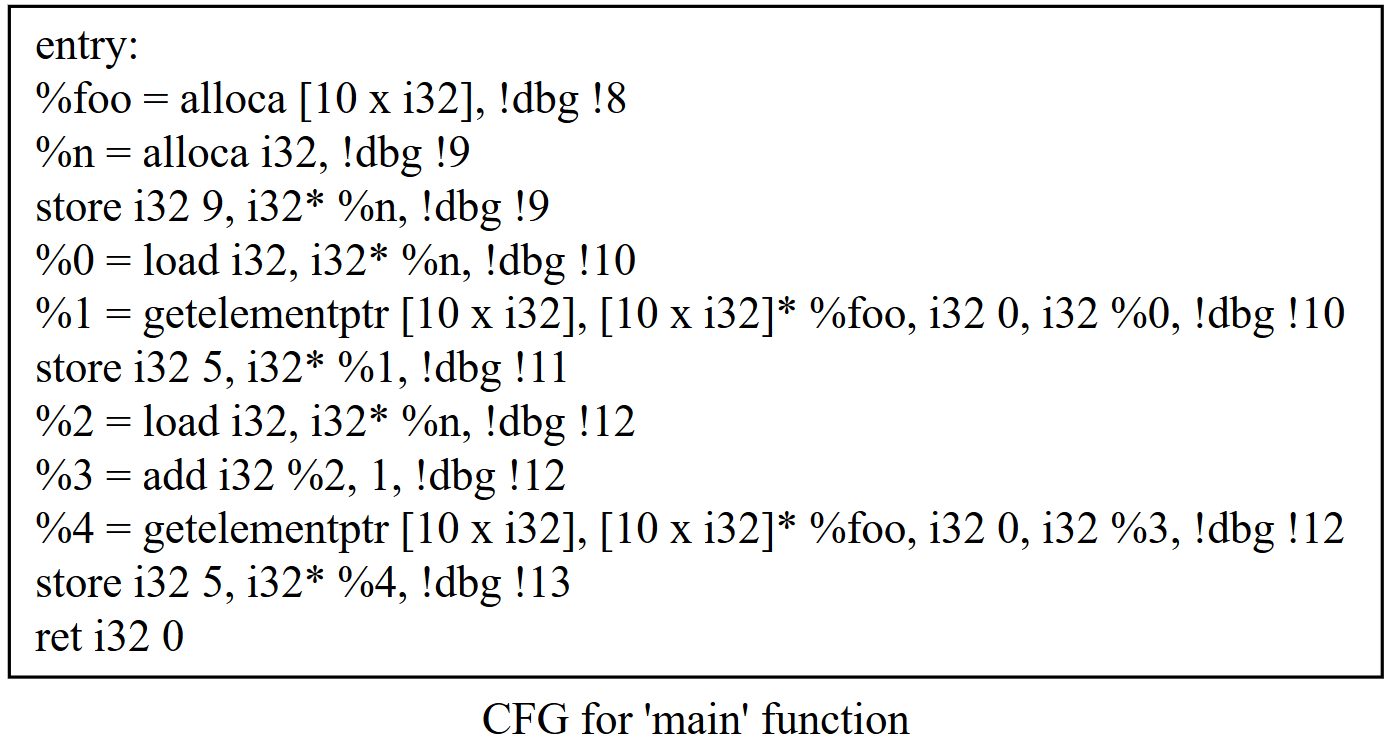
\includegraphics[width=\linewidth]{fig_overflow}
	\end{minipage}
\end{figure}

This program results in the IR shown in figure 
\begin{figure}
	content...
\end{figure}
	\section{Analysis}
	To perform the analysis, the program \texttt{bubble\_sort.c} is executed 30 times for each representation. Afterwards, average statistics such as runtime can be calculated for each representation. It can be assumed that inserting more code to perform the runtime boundchecking will increase performance overhead. Indeed, table \ref{table:1} shows that applying runtime bounds checking increases the runtime by an average of 13\%. This has a straightforward explanation: each \texttt{getelementptr} gets preceded by a \texttt{cmp} and \texttt{br} instruction.
	
	\begin{table}
		\centering
		\begin{tabular}{ l | l | l |}
			& Original IR & IR with bounds checking \\
			Average runtime & 2758 ms & 3141 ms
		\end{tabular}
		\label{table:1}
	\end{table}
	
	
	
	
\end{document}